\documentclass[11pt]{article}
\usepackage{fontspec}
\usepackage{polyglossia}
\setmainlanguage{spanish}
\usepackage[a4paper,margin=2.2cm]{geometry}
\usepackage{amsmath,amssymb}
\usepackage{graphicx}
\usepackage{booktabs}
\usepackage{array}
\usepackage{float}
\usepackage[font=small,labelfont=bf]{caption}
\usepackage{enumitem}
\usepackage{xcolor}
\usepackage[most]{tcolorbox}
\usepackage{tikz}
\usetikzlibrary{arrows.meta,positioning,calc}
\usepackage{hyperref}
\hypersetup{colorlinks=true,linkcolor=azul,urlcolor=azul}
\usepackage{fancyhdr}
\usepackage{titlesec}

\definecolor{azul}{HTML}{1F4E79}
\definecolor{gris}{HTML}{F2F4F7}
\definecolor{rojo}{HTML}{C0504D}

\titleformat{\section}{\large\bfseries\color{azul}}{\thesection.}{0.6em}{}
\titleformat{\subsection}{\normalsize\bfseries\color{azul}}{\thesubsection}{0.6em}{}
\setlength{\parskip}{0.45em}
\setlength{\parindent}{0pt}
\setlist{itemsep=0.15em,topsep=0.3em}

\newtcolorbox{clave}[1][]{colback=gris,colframe=azul,boxrule=0.6pt,arc=2pt,left=6pt,right=6pt,top=4pt,bottom=4pt,fonttitle=\bfseries\small,title={#1}}
\newtcolorbox{alerta}[1][]{colback=rojo!6,colframe=rojo,boxrule=0.6pt,arc=2pt,left=6pt,right=6pt,top=4pt,bottom=4pt,fonttitle=\bfseries\small,title={#1}}

\pagestyle{fancy}
\fancyhf{}
\renewcommand{\headrulewidth}{0.4pt}
\fancyfoot[C]{\small\thepage}

\fancyhead[L]{\small Justificación — SCARA con observadores, ESP32 y micro-ROS}
\fancyhead[R]{\small Universidad EIA}
\newtcolorbox{preg}[1][]{colback=white,colframe=azul!55,boxrule=0.5pt,arc=2pt,left=6pt,right=6pt,top=3pt,bottom=3pt,fonttitle=\bfseries\small,title={#1},breakable}
\newcommand{\cod}[1]{\texttt{#1}}

\begin{document}

\begin{center}
{\LARGE\bfseries\color{azul} Justificación del sistema de control del robot SCARA}\\[0.4em]
{\large Observadores de Luenberger y Kalman en el ESP32, PID con el modelo identificado,\\ manejo de motores y panel de control con ROS 2 y micro-ROS}\\[0.6em]
{\small Juan David Botero · Universidad EIA · octubre de 2026 · código: rama \cod{observadores-panel} de \cod{SCARA\_PROCCES}}
\end{center}

\begin{clave}[Resumen en una tabla]
\small
\begin{tabular}{@{}>{\raggedright\arraybackslash}p{4.3cm}>{\raggedright\arraybackslash}p{11.4cm}@{}}
Arquitectura & ESP32 (ESP-IDF 5.3): control a 1 kHz, observadores a 100 Hz, telemetría a 20 Hz. PC con Ubuntu y ROS 2 Jazzy: panel. Enlace micro-ROS por USB. \\
Modelo del motor & El del Laboratorio 4 (Pololu 37D, 100:1), referido al eje de salida: a 12 V da 114,3 rpm y 0,200 A. \\
Observadores & Luenberger (polos $0{,}25\pm0{,}25j$) y Kalman ($K_w\to0{,}266$) para los 3 motores; idénticos al MATLAB del laboratorio (diferencia máxima $2\times10^{-5}$ rpm con los datos reales). \\
PID & J1: diseñado por ubicación de polos con el modelo (5350 · 18500 · 295). J2: las del Reporte 3 (5000 · 3000 · 180), porque con las del modelo quedó muy agresivo en el robot. \\
Motores & Cada motor se habilita o deshabilita en cualquier momento; potencia manual en lazo abierto, de 0 a 100 \%, con dead-man. \\
Validación & 149 comprobaciones automáticas en el PC. Con las ganancias originales, la simulación original da exactamente la misma salida que el código de antes. Cargado y probado en el ESP32. \\
\end{tabular}
\end{clave}

%=====================================================================
\section{Qué se pidió y cómo se cumple}

\begin{table}[H]\centering\small
\begin{tabular}{>{\raggedright\arraybackslash}p{4.6cm}>{\raggedright\arraybackslash}p{11cm}}
\toprule
Requisito & Cómo se cumple \\
\midrule
Linux y micro-ROS & El ESP32 es un nodo micro-ROS (\cod{/scara/scara\_esp32}) conectado al agente en Docker; el PC usa ROS 2 Jazzy en Ubuntu. \\
Monitorear velocidad, corriente, observadores, $P$ y $K$ & Tópico nuevo \cod{/scara/obs} con 12 datos por motor (medida, Luenberger, Kalman a priori y a posteriori, $\sqrt{P}$, $K$, voltaje del modelo) y gráficas en el panel. \\
Activar y desactivar cualquier motor & Interruptor por motor en el panel, o \cod{motor j on|off} y \cod{motors a b c}. \\
Controladores ``de verdad'' con los datos identificados & Observadores y PID calculados con el modelo identificado del Laboratorio 4, no con la hoja de datos. \\
Manejar a mano la potencia & Modo Potencia: un deslizador de 0 a 100 \% y sentido por motor, aplicado mientras se mantiene el dead-man. \\
Interfaz más bonita & Panel nuevo en PyQt5 + pyqtgraph (tema oscuro, tarjetas por motor, 4 pestañas, registro, CSV, modo demo). \\
Documentación & README reorganizado, \cod{UBUNTU\_MICROROS.md}, guía de operación en PDF y este documento. \\
\bottomrule
\end{tabular}
\end{table}

%=====================================================================
\section{Arquitectura: qué corre dónde y por qué}

\begin{figure}[H]\centering
\begin{tikzpicture}[font=\small, node distance=4mm,
  caja/.style={draw=azul, rounded corners=2pt, fill=gris, align=center, inner sep=4pt, font=\footnotesize},
  flecha/.style={-{Stealth[length=2mm]}, thick, azul}]
\node[caja, text width=6.0cm] (esp) {\textbf{ESP32} (tiempo real)\\[2pt]
  lazo de control a 1~kHz: PID, rampa,\\ seguridad, Home\\ observadores a 100 Hz:\\ Luenberger + Kalman (×3)\\ cinemática inversa, trayectorias};
\node[caja, right=3.4cm of esp, text width=4.0cm] (pc) {\textbf{PC con Ubuntu}\\[2pt] ROS 2 Jazzy\\ panel PyQt5\\ (gráficas, dead-man)\\ RViz, scripts};
\node[caja, below=7mm of esp, text width=6.0cm] (hw) {TB6612 (PWM 20~kHz) · 3 motores\\ Pololu 37D · encoders (PCNT)\\ 4 finales de carrera};
\draw[flecha, <->] (esp) -- node[above, align=center, font=\scriptsize]{micro-ROS (XRCE-DDS)\\ USB 115200 baudios} node[below, font=\scriptsize]{agente en Docker} (pc);
\draw[flecha, <->] (esp) -- (hw);
\end{tikzpicture}
\caption{El control y la seguridad viven en el ESP32; ROS 2 solo manda consignas y recibe estado.}
\end{figure}

\begin{itemize}
  \item \textbf{El lazo de control no pasa por ROS.} Un lazo de 1 kHz necesita un período fijo; por USB y DDS hay latencia y variación de varios milisegundos. Además, si el PC se cuelga o se cae el cable, el robot debe seguir siendo seguro por sí solo.
  \item \textbf{Calidad de servicio (QoS).} Los flujos periódicos (\cod{state}, \cod{obs}, \cod{jog}, \cod{power}, \cod{ee\_position}) son \emph{best-effort}: si se pierde un dato, el siguiente llega en 40--50 ms y reenviarlo solo retrasaría la cola. Las órdenes y eventos (\cod{goto}, \cod{cmd}, \cod{event}) son \emph{reliable}: una orden no se puede perder.
  \item \textbf{Ancho de banda.} \cod{/scara/obs} (38 números) y \cod{/scara/state} (19) a 20 Hz ocupan cerca del 55 \% de 115200 baudios. Si se quieren gráficas más fluidas se sube a 460800 baudios.
  \item \textbf{Mensajes estándar.} Se usan \cod{Float32MultiArray}, \cod{Point}, \cod{Vector3} y \cod{String}: un mensaje propio obligaría a recompilar la librería micro-ROS con un paquete de interfaces. El orden de los datos está documentado en \cod{ros2/scara\_common.py}. Los 13 primeros datos de \cod{/scara/state} son los de siempre, así los scripts anteriores siguen funcionando.
\end{itemize}

%=====================================================================
\section{Modelo del motor}

Se usa el modelo ajustado en el Laboratorio 4 ($R_a$ y $L_a$ medidos; $K_v$, $\beta$ y $J$ ajustados para que a 12 V el motor dé 0,2 A y 114,3 rpm con la dinámica medida). En el firmware está \textbf{referido al eje de salida} del reductor ($K_v\cdot N$, $\beta\cdot N^2$, $J\cdot N^2$): así las unidades son las de la articulación y no depende de si la caja es 100,37:1 o 102,08:1.
\begin{equation}
L_a\frac{di}{dt}=V-R_a i-K_v\omega,\qquad J\frac{d\omega}{dt}=K_v i-\beta\omega,\qquad y=\omega
\end{equation}

\begin{table}[H]\centering\small
\begin{tabular}{lccccc}
\toprule
 & $R_a$ [$\Omega$] & $L_a$ [H] & $K_v$ [V·s/rad] & $\beta$ [N·m·s/rad] & $J$ [kg·m²] \\
\midrule
Eje de salida (firmware) & 50 & 0,060 & 0,167092 & $2{,}792\times10^{-3}$ & $3{,}632\times10^{-4}$ \\
\bottomrule
\end{tabular}
\end{table}

Polos continuos: $-831{,}8$ s$^{-1}$ (eléctrico, $\tau=1{,}2$ ms) y $-9{,}24$ s$^{-1}$ (mecánico, $\tau=108$ ms). En régimen permanente a 12 V el modelo da 114,30 rpm y 0,2000 A.

\textbf{Voltaje que recibe el motor.} El observador necesita el voltaje real, no el PWM. Se modela con una ganancia y una zona muerta:
\begin{equation}
V = g\,(12\ \text{V}\cdot d) - \operatorname{signo}(d)\,v_0,\qquad V=0 \text{ si } |g\,12\,d|<v_0
\end{equation}
Con el L298N del laboratorio se midió $g=0{,}9782$ y $v_0=1{,}197$ V (caída de sus transistores bipolares). La tarjeta usa un TB6612 (MOSFET, caída casi nula): $g=1$ y $v_0\approx0{,}8$ V, que equivale a la fricción seca que el PID compensa con \cod{fric} $=70$ (70/1023·12 V $=0{,}82$ V). Se puede cambiar en vivo con \cod{vmap g v0}.

%=====================================================================
\section{Observadores en el ESP32}

\subsection*{Período de muestreo: 10 ms (no 1 ms)}
La velocidad se mide como diferencia de cuentas del encoder (6424 por vuelta de salida). Una cuenta en 10 ms equivale a $60/(0{,}01\cdot6424)=0{,}93$ rpm; en 1 ms equivaldría a 9,3 rpm, una medida inútilmente gruesa. Con 10 ms además se usan los mismos $T_s$, $R$ y polos del laboratorio. Los observadores corren cada 10 ticks del lazo de 1 kHz; como el PWM cambia cada 1 ms, la entrada del observador es el \textbf{voltaje medio} del intervalo, que es lo que exige el modelo discreto: $x_k=A\,x_{k-1}+B\,u_{k-1}$ con $u$ constante en el intervalo.

\subsection*{Discretización exacta (ZOH)}
\begin{equation}
\begin{bmatrix}A & B\\ 0 & 1\end{bmatrix}=\exp\!\left(\begin{bmatrix}A_c & B_c\\ 0 & 0\end{bmatrix}T_s\right),\qquad
A=\begin{bmatrix}-0{,}00148 & -0{,}00309\\ 0{,}50976 & 0{,}91345\end{bmatrix},\quad B=\begin{bmatrix}0{,}01977\\ 0{,}07783\end{bmatrix}
\end{equation}
La exponencial se calcula en el propio ESP32 (escalado y elevación al cuadrado + serie de Taylor), así un cambio de parámetros no requiere MATLAB. \textbf{No se usa Euler:} con el polo eléctrico, $1+\lambda T_s=1-831{,}8\cdot0{,}01=-7{,}3$, fuera del círculo unitario; Euler daría un modelo discreto inestable.

\subsection*{Observabilidad}
Solo se mide la velocidad, $C=[0\ \ 1]$:
\begin{equation}
\mathcal O=\begin{bmatrix}C\\ CA\end{bmatrix}=\begin{bmatrix}0 & 1\\ 0{,}5098 & 0{,}9135\end{bmatrix},\qquad \det\mathcal O=-0{,}51\neq0 \Rightarrow \operatorname{rango}=2
\end{equation}
La corriente se ``ve'' a través de la velocidad porque produce el par ($A_{21}\neq0$).

\subsection*{Luenberger}
$\hat x_k=A\hat x_{k-1}+Bu_{k-1}+L\,(y_{k-1}-C\hat x_{k-1})$. Con Ackermann y $C=[0\ 1]$: $L=\phi(A)\,e_1/A_{21}$, con $\phi(z)$ el polinomio deseado.
\begin{itemize}
  \item Polos $0{,}25\pm0{,}25j$ (los del laboratorio): $|z|=0{,}354$, constante de tiempo $-T_s/\ln|z|=9{,}6$ ms, unas 10 veces más rápido que el polo mecánico de la planta ($z=0{,}912$, 108 ms). Converge en 3--4 muestras.
  \item Resultado: $L=[0{,}2436\ \ 0{,}4120]^T$ (A y rad/s por rad/s de error). Se comprobó que los polos de $A-LC$ son exactamente $0{,}25\pm0{,}25j$.
  \item Precio: un observador rápido confía mucho en la medida, así que el ruido de cuantización pasa a la corriente estimada.
\end{itemize}

\subsection*{Kalman}
\begin{align}
\text{Predicción:}\quad & \hat x^-_k=A\hat x_{k-1}+Bu_{k-1}, \qquad P^-_k=AP_{k-1}A^T+Q\\
\text{Corrección:}\quad & K_k=P^-_kC^T(CP^-_kC^T+R)^{-1},\quad \hat x_k=\hat x^-_k+K_k(y_k-C\hat x^-_k),\quad P_k=(I-K_kC)P^-_k
\end{align}
\begin{itemize}
  \item $R=\sigma_y^2=(0{,}81\ \text{rpm})^2=0{,}655$ rpm²: \textbf{medido} en el laboratorio con el motor a velocidad constante.
  \item $Q=\operatorname{diag}(\sigma_i^2,\sigma_\omega^2)$ con $\sigma_i=10$ mA y $\sigma_\omega=0{,}30$ rpm: cuánto se desconfía del modelo; son los del laboratorio.
  \item $P_0=\operatorname{diag}(0{,}1\ \text{A},\ 1\ \text{rpm})^2$. En el primer paso se toma $\hat x=0$, $P=P_0$ sin corregir, igual que en MATLAB.
  \item En estado estable: $K_w=0{,}266$, $K_i=-5{,}6\times10^{-4}$ A/(rad/s), $\sqrt{P_\omega}=0{,}42$ rpm, $\sqrt{P_i}=10$ mA.
  \item Se calcula en línea (matrices 2×2, unas decenas de operaciones por motor cada 10 ms), así el panel puede mostrar cómo convergen $P$ y $K$ y se pueden cambiar $Q$ y $R$ en vivo con \cod{kal}.
  \item El motor 3, si no tiene encoder, corre solo con el modelo (sin corrección).
\end{itemize}

\subsection*{Validación}
\begin{itemize}
  \item El código C da los mismos $A$, $B$, $L$ y $K$ que el laboratorio y, con los datos reales del laboratorio, la misma salida que el MATLAB (diferencia máxima $2\times10^{-5}$ rpm).
  \item Simulación con la planta identificada y el encoder cuantizado (figura \ref{fig:obs}). Error RMS de velocidad: medida 0,40 rpm, Luenberger 0,13 rpm, Kalman 0,087 rpm. Corriente: Luenberger 12,6 mA de ruido, Kalman prácticamente exacto. Aquí el Kalman conoce la planta exacta; en el robot el error de corriente será mayor (ver limitaciones).
\end{itemize}

\begin{figure}[H]\centering
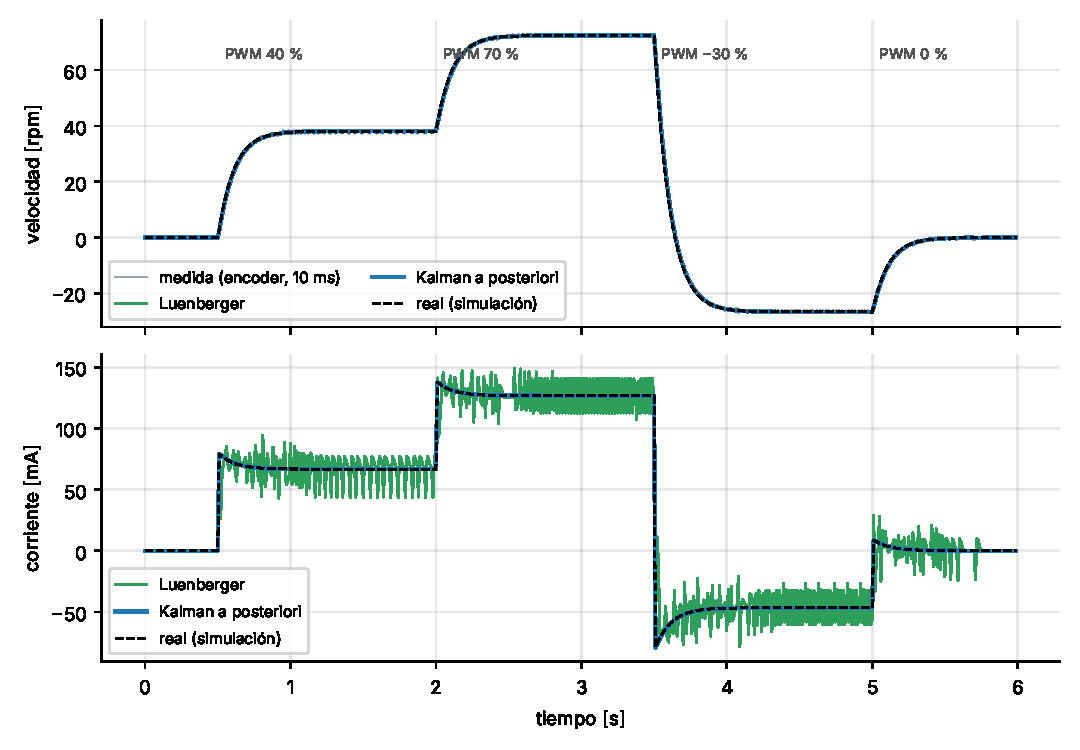
\includegraphics[width=0.92\linewidth]{figs/f_observadores.pdf}
\caption{Simulación: escalones de PWM (40, 70, $-30$, 0 \%) con la planta identificada, zona muerta de 0,8 V y encoder de 6424 cuentas leído cada 10 ms. En velocidad las curvas casi coinciden; en corriente se ve que el Luenberger deja pasar el ruido de cuantización y el Kalman no.}
\label{fig:obs}
\end{figure}

%=====================================================================
\section{PID de posición}

\subsection*{Diseño con el modelo (J1)}
Con $L_a$ despreciable (polo de 1,2 ms frente a 108 ms), la planta de posición es
\begin{equation}
\frac{\theta(s)}{V(s)}=\frac{K}{s(\tau s+1)},\qquad K=\frac{K_v}{R_a\beta+K_v^2}=0{,}9974\ \tfrac{\text{rad/s}}{\text{V}},\quad \tau=\frac{JR_a}{R_a\beta+K_v^2}=0{,}108\ \text{s}
\end{equation}
Con $u=K_p e+K_i\!\int\! e-K_d\dot\theta$, la ecuación característica es $\tau s^3+(1+KK_d)s^2+KK_ps+KK_i=0$. Se iguala a
\begin{equation}
(s^2+2\cdot0{,}9\cdot20\,s+20^2)(s+5)
\end{equation}
$\zeta=0{,}9$ (casi sin sobrepaso), $\omega_n=20$ rad/s (unas 2 veces más rápido que la planta, sin pedir más de lo que el PWM puede dar) y un polo en $-5$ para la integral. Resulta $K_p=62{,}8$ V/rad, $K_i=216{,}6$ V/(rad·s), $K_d=3{,}44$ V·s/rad; en unidades de PWM ($\times1023/12$): \textbf{kp = 5350, ki = 18500, kd = 295}. La prealimentación es $k_{ff}=1/K$: 85.

Además el PID del firmware tiene: anti-windup (no integra si está saturado empujando hacia el mismo lado, e integral limitada a 250), compensación de fricción seca (\cod{fric} $=70$ fuera de una zona de $0{,}15^\circ$), derivada sobre la velocidad medida (no sobre el error, para no dar golpes en un cambio de consigna), rampa de PWM de 0,34 s a fondo de escala y tope del 63 \%.

\subsection*{Por qué J2 usa las ganancias del Reporte 3}
En el robot, con las ganancias del modelo, \textbf{el eslabón 2 quedó muy agresivo}. Se volvió a las del Reporte 3 (5000 · 3000 · 180 · 80 · 70), que ya estaban probadas en ese eje. Explicación:
\begin{itemize}
  \item La diferencia principal es la integral: $k_i$ es 6 veces mayor. En lazo cerrado las del modelo ponen los polos en $-18{,}0\pm8{,}4j$ y $-5{,}0$; las del Reporte 3 en $-14{,}0\pm18{,}1j$ y $-0{,}62$, es decir, una integral mucho más lenta y suave.
  \item El cero que agrega la integral ($k_i/k_p=3{,}5$ frente a 0,6) produce más sobrepaso: en el análisis lineal (figura \ref{fig:pid}) un escalón de $2^\circ$ da 20 \% con las del modelo y 13 \% con las del Reporte 3.
  \item El modelo se identificó con el motor solo en el banco y con un L298N. El eslabón 2 es liviano y tiene fricción, juego de la caja y cuantización del encoder que el modelo no incluye; con una integral fuerte, esas no linealidades hacen que el PWM suba y el eje ``busque'' la posición.
\end{itemize}
J1 conserva las del modelo. Las ganancias se cambian en vivo (\cod{gain j kp ki kd kff fric} o la pestaña Sintonía) y se dejan fijas en \cod{src/config.c}.

\begin{figure}[H]\centering
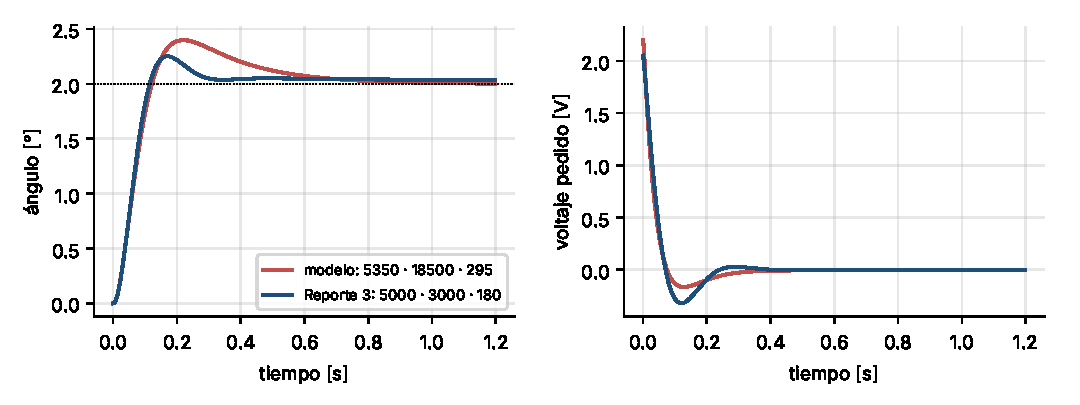
\includegraphics[width=0.92\linewidth]{figs/f_pid.pdf}
\caption{Análisis lineal (modelo identificado, lazo de 1 kHz, sin saturación ni zona muerta): escalón de $2^\circ$ con las dos ganancias. En el robot los movimientos usan trayectorias suaves con prealimentación, no escalones; la figura sirve para comparar la agresividad de cada juego.}
\label{fig:pid}
\end{figure}

%=====================================================================
\section{Habilitar y deshabilitar motores}

\begin{table}[H]\centering\small
\begin{tabular}{>{\raggedright\arraybackslash}p{3.6cm}>{\raggedright\arraybackslash}p{12cm}}
\toprule
Un motor deshabilitado & Por qué \\
\midrule
Driver libre (IN1 = IN2 = 0) & Se puede mover el eslabón a mano y no consume. \\
El encoder sigue contando & No se pierde el Home: al rehabilitarlo la posición sigue siendo válida. \\
Home solo de los habilitados & Permite probar un eje sin mover el otro. \\
\cod{goto x y z} exige J1 y J2 & La cinemática inversa usa los dos ángulos; mover solo uno no llevaría al punto. \\
\cod{ang q1 q2} mueve solo los habilitados & Mover articulaciones sueltas sí tiene sentido. \\
Fuera de la supervisión de fallas & Si alguien lo mueve a mano no debe disparar ``error de seguimiento''. \\
Al rehabilitarlo, mantiene su posición & No da un salto hacia una referencia vieja. \\
\bottomrule
\end{tabular}
\end{table}
Al encender están habilitados M1 y M2 y el M3 (atornillador) deshabilitado, igual que antes del cambio.

%=====================================================================
\section{Potencia manual (lazo abierto)}

\begin{itemize}
  \item \textbf{Dead-man.} El panel manda \cod{/scara/power = [dead-man, \%M1, \%M2, \%M3]} a 25 Hz. Sin latidos durante 300 ms (unos 7 latidos perdidos) todo vuelve a 0. Por USB-serial en modo texto el plazo es 150 ms; con micro-ROS se dio más margen por la variación de latencia de DDS. Si el agente se desconecta, el ESP32 apaga la potencia y el jog.
  \item \textbf{Al soltar}, cada eje frena con amortiguamiento ($u=-k_d\,\dot q$) hasta $|\dot q|<0{,}03$ rad/s y luego queda en HOLD con su PID, donde paró. Volver a la referencia vieja sería un salto inesperado.
  \item \textbf{Bloqueo.} DETENER, APAGAR o una falla bloquean la potencia hasta que se suelte el dead-man, para que no arranque sola otra vez.
  \item \textbf{Límites que se mantienen:} tope de 63 \% de PWM, rampa, no empujar contra un final de carrera presionado, límites por software si hay Home, y detección de motor trabado.
  \item \textbf{M3 (atornillador)} solo se mueve en este modo y funciona en paralelo con el brazo.
\end{itemize}

\textbf{Escala de 0 a 100 \%.} Por debajo de unos 7 \% de PWM el motor no se mueve (zona muerta), y un eje puede necesitar mucho menos que el tope para moverse bien. Por eso el deslizador no manda el PWM directo:
\begin{equation}
d=\begin{cases}0 & p=0\\ \operatorname{signo}(p)\left[d_{arr}+(d_{tope}-d_{arr})\frac{|p|}{100}\right] & p\neq0\end{cases}
\end{equation}
con $d_{arr}=7$ \% (apenas arranca) y $d_{tope}$ = 60 \% (M1, M3) y 30 \% (M2). Todo el recorrido del deslizador es útil y el eslabón 2 no recibe más potencia de la necesaria. Por \cod{/scara/power} sigue viajando PWM real; la escala es solo del panel.

%=====================================================================
\section{Corriente estimada frente a la fuente}

La corriente del observador es la del \emph{motor}. La fuente ve otra cosa. Por balance de potencia en el puente H (pérdidas despreciables), $V_{bus}\,I_{in}=V_{motor}\,i=(d\,V_{bus})\,i$, de modo que
\begin{equation}
I_{fuente}\approx I_{lógica}+\sum_m |i_m|\,|d_m|
\end{equation}
$I_{lógica}$ es el consumo del ESP32, reguladores, encoders y driver; se mide en la fuente con los motores apagados y se escribe en el panel. Ejemplo: en el robot se vio 0,05 A estimados en el motor frente a 0,114 A en la fuente; la mayor parte de la diferencia es la parte lógica, y con PWM parcial la fuente ve aún menos de la corriente del motor. El panel muestra el valor estimado de la fuente para compararlo con el amperímetro.

%=====================================================================
\section{Panel de control}

\begin{figure}[H]\centering
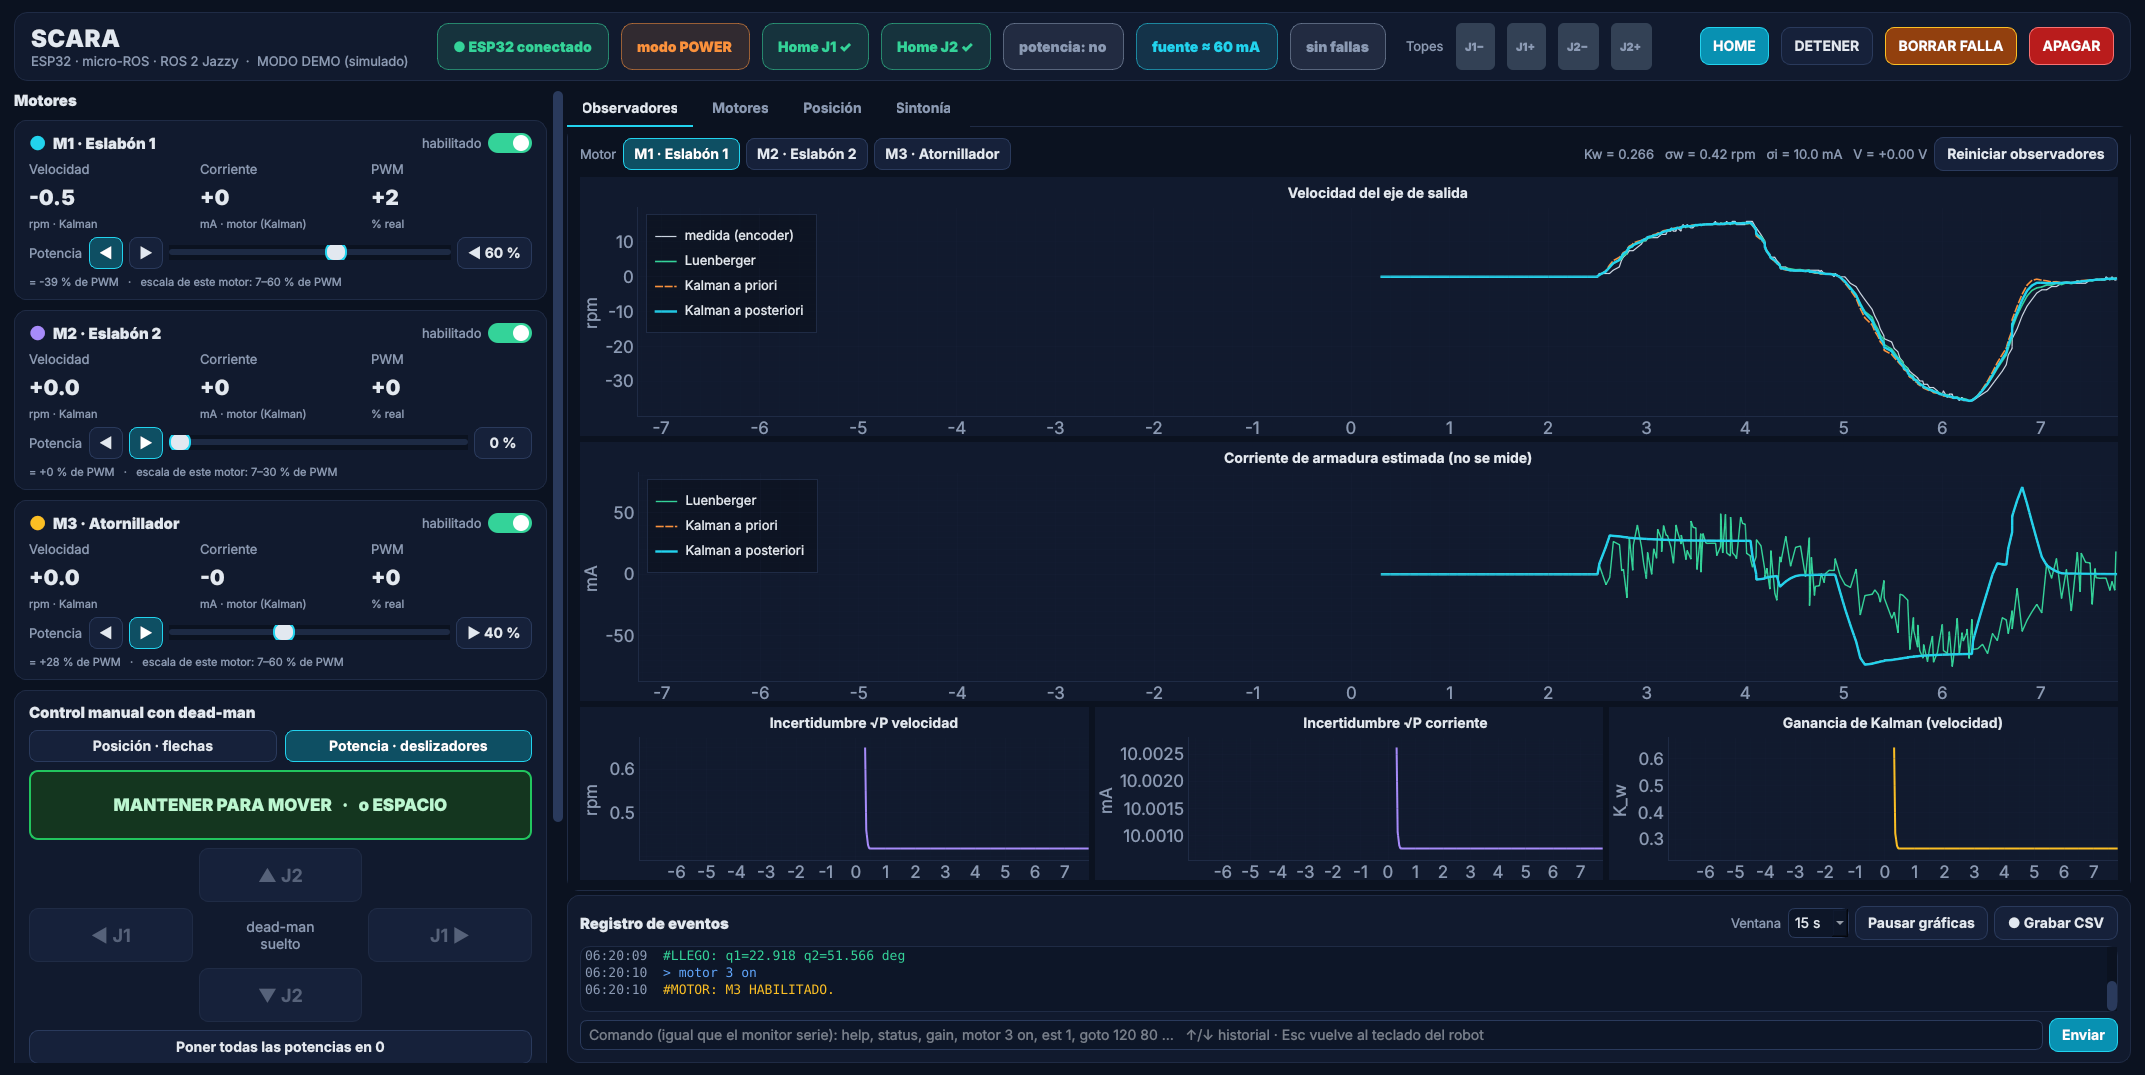
\includegraphics[width=\linewidth]{../img/panel_observadores.png}
\caption{Pestaña Observadores: velocidad medida, Luenberger, Kalman a priori y a posteriori; corriente estimada; $\sqrt P$ y $K_w$. A la izquierda, las tarjetas de los motores con su interruptor y su deslizador de potencia.}
\end{figure}
\begin{itemize}
  \item \textbf{PyQt5 + pyqtgraph}: gráficas en tiempo real fluidas (pyqtgraph dibuja con Qt, no con matplotlib) y ventana nativa. rclpy corre en un hilo aparte para que la interfaz no se congele.
  \item \textbf{Seguridad}: si la ventana pierde el foco o se escribe en un cuadro de texto, el dead-man se suelta; se ignora la auto-repetición del teclado.
  \item \textbf{Modo demo} (\cod{--demo}): simula el ESP32 con el mismo modelo y una copia en Python de los observadores; sirve para practicar la presentación sin el robot.
  \item \textbf{CSV}: graba todas las estimaciones a 20 Hz para analizarlas después en MATLAB.
\end{itemize}

%=====================================================================
\section{Cómo se comprobó que no se dañó lo que ya funcionaba}

\begin{itemize}
  \item \textbf{Regresión.} Se corrieron las pruebas \emph{originales} (sin modificarlas, salvo agrandar sus arreglos de 2 a 3 motores y agregar funciones vacías para las órdenes nuevas) contra el código nuevo. Con las ganancias originales, la simulación de Home, \cod{goto}, manual, límites y fallas da \textbf{exactamente la misma salida} que el código anterior, línea por línea. Los comandos de texto y de ROS dan el mismo resultado.
  \item \textbf{Sin tocar:} pines de M1 y M2, límites, cinemática, trayectorias, PID y \cod{main}.
  \item \textbf{Pruebas nuevas:} 149 comprobaciones (estimador contra el laboratorio, simulación completa con dos plantas, comandos, formato de tópicos, escala de potencia y corriente de la fuente).
  \item \textbf{En el robot:} el firmware se compiló y cargó en el ESP32 y se probó con el panel; de ahí salió el ajuste de J2.
\end{itemize}

%=====================================================================
\section{Limitaciones y cómo las defendemos}

\begin{alerta}[Lo que hay que decir antes de que lo pregunten]
\begin{itemize}
  \item \textbf{La corriente no se mide, se estima.} El sensado de corriente de la tarjeta no está activo. La estimación depende del modelo; con $R_a=50~\Omega$ (medido en el laboratorio, alto para este motor) el modelo da poco par por amperio y subestima la corriente con carga. Sirve para ver tendencias, no como medida exacta.
  \item \textbf{El modelo se identificó con el motor solo y con un L298N;} el robot usa un TB6612 y tiene eslabones. Por eso $v_0=0{,}8$ V es una estimación y J2 necesitó otras ganancias.
  \item \textbf{La medida de velocidad es un promedio en 10 ms} (diferencia de cuentas), no la velocidad instantánea: tiene medio período de retraso. Es la misma convención del laboratorio.
  \item \textbf{Pendientes de confirmar en el hardware:} pines del encoder de M3 (32 y 14 en J8) y sus signos.
\end{itemize}
\end{alerta}

%=====================================================================
\section{Preguntas probables y respuestas}

\begin{preg}[1. ¿Para qué observadores si el encoder ya mide la velocidad?]
Por dos razones. La corriente no se está midiendo (el sensado de corriente de la tarjeta no está activo) y los observadores la estiman a partir de la velocidad; es la base para el control de par del atornillador ($\tau=K_v\,i$, con $K_v=0{,}167$ N·m/A en el eje de salida). Y la velocidad del encoder llega en escalones de 0,93 rpm; el Kalman la filtra (error RMS de 0,40 a 0,087 rpm en simulación).
\end{preg}

\begin{preg}[2. ¿Cómo saben que el sistema es observable midiendo solo la velocidad?]
$\mathcal O=[C;\,CA]$ tiene determinante $-0{,}51$, rango 2. Físicamente: la corriente produce par, el par cambia la velocidad, y la velocidad se mide.
\end{preg}

\begin{preg}[3. ¿Por qué 10 ms y no el 1 ms del lazo de control?]
Por resolución: una cuenta en 1 ms son 9,3 rpm; en 10 ms, 0,93 rpm. Y así se conservan el $T_s$, la $R$ medida y los polos del laboratorio. El PID sigue a 1 kHz.
\end{preg}

\begin{preg}[4. ¿Por qué discretizaron con la exponencial y no con Euler?]
Con $T_s=10$ ms y el polo eléctrico en $-831{,}8$, Euler da $1-8{,}3=-7{,}3$: un polo discreto fuera del círculo unitario, modelo inestable. La exponencial (ZOH) es exacta para entrada constante en el intervalo.
\end{preg}

\begin{preg}[5. ¿Por qué esos polos del Luenberger?]
$0{,}25\pm0{,}25j$ ($|z|=0{,}35$): converge en 3--4 muestras, unas 10 veces más rápido que la planta. Más rápido amplifica más el ruido de cuantización en la corriente; más lento tarda en seguir los cambios. Son los del laboratorio y se pueden cambiar en vivo con \cod{luen}.
\end{preg}

\begin{preg}[6. ¿Qué diferencia hay entre Kalman a priori y a posteriori?]
A priori es la predicción del modelo antes de ver la medida ($\hat x^-=A\hat x+Bu$); a posteriori es la predicción corregida con la medida ($\hat x=\hat x^-+K(y-C\hat x^-)$). En la gráfica, la a priori va un poco por detrás y la a posteriori se acerca a la medida filtrada.
\end{preg}

\begin{preg}[7. ¿De dónde salen Q y R?]
$R=0{,}655$ rpm² se midió en el laboratorio (varianza de la velocidad medida a velocidad constante). $Q$ expresa cuánto se desconfía del modelo (10 mA en corriente, 0,30 rpm en velocidad); se eligió en el laboratorio comparando con los datos. Subir $Q$ hace al filtro más rápido y más ruidoso; subir $R$, más lento y más suave.
\end{preg}

\begin{preg}[8. ¿Por qué el Kalman tiene menos ruido en la corriente que el Luenberger?]
El Luenberger usa una $L$ fija y grande (polos rápidos), así que todo el ruido de la medida pasa al estado. El Kalman pondera: como la medida es ruidosa ($R$) y el modelo es bueno ($Q$ pequeño), $K_i$ es casi cero y la corriente sale casi solo del modelo.
\end{preg}

\begin{preg}[9. ¿La ganancia del Kalman cambia en el tiempo?]
Sí, al principio: parte de $P_0$ y converge en pocas muestras a $K_w=0{,}266$. Se calcula en línea para poder mostrar esa convergencia en el panel y cambiar $Q$ y $R$ sin recompilar; en estado estable equivale a un filtro de ganancia fija.
\end{preg}

\begin{preg}[10. ¿Por qué la corriente estimada no coincide con la fuente?]
Porque no miden lo mismo: la fuente suma la parte lógica y, con PWM, solo ve la corriente del motor el tiempo encendido ($I_{fuente}\approx I_{lógica}+\sum|i|\,d$). El resto de la diferencia es el modelo ($R_a=50~\Omega$).
\end{preg}

\begin{preg}[11. ¿Por qué el control está en el ESP32 y no en ROS?]
El lazo de 1 kHz necesita un período fijo y la seguridad no puede depender del PC ni del cable. ROS solo manda consignas y recibe estado; si se pierde el enlace, el ESP32 se detiene solo.
\end{preg}

\begin{preg}[12. ¿Qué pasa si se desconecta el cable o se cae el agente?]
Sin latidos durante 300 ms el modo manual y la potencia vuelven a 0. Además el ESP32 hace ping al agente cada segundo; si no responde, apaga jog y potencia, destruye las entidades y espera a que vuelva el agente. El brazo queda en HOLD.
\end{preg}

\begin{preg}[13. ¿Por qué best-effort en unos tópicos y reliable en otros?]
Los periódicos se reemplazan cada 40--50 ms: reenviar uno viejo no sirve y llena la cola. Una orden (\cod{goto}, \cod{cmd}) o un evento no se puede perder.
\end{preg}

\begin{preg}[14. ¿Cómo diseñaron el PID?]
Ubicación de polos sobre $K/(s(\tau s+1))$ con $K=0{,}9974$ y $\tau=0{,}108$: se iguala la ecuación característica a $(s^2+36s+400)(s+5)$. Se le añaden prealimentación de velocidad ($1/K$), compensación de fricción y anti-windup.
\end{preg}

\begin{preg}[15. ¿Por qué el eslabón 2 tiene otras ganancias que el 1?]
En el robot quedó muy agresivo con las del modelo. La causa principal es la integral (6 veces mayor), que con la fricción, el juego y la cuantización hace que el PWM suba y el eje busque la posición. El modelo se identificó con el motor solo, sin eslabón. Se dejaron las del Reporte 3, ya probadas en ese eje; J1 conserva las del modelo.
\end{preg}

\begin{preg}[16. ¿Qué hacen kff y fric?]
\cod{kff} da de una vez el PWM que la trayectoria necesita para su velocidad ($1/K$), así el PID solo corrige el error. \cod{fric} suma el PWM que vence la fricción seca (unos 0,8 V) cuando hay error, para que el eje no se quede pegado cerca de la consigna.
\end{preg}

\begin{preg}[17. ¿Qué es el anti-windup?]
Si el PWM está saturado empujando hacia el lado del error, se deja de integrar; además la integral está limitada a 250. Sin eso, la integral crece durante la saturación y produce un sobrepaso grande al salir.
\end{preg}

\begin{preg}[18. ¿Qué pasa si deshabilito un motor en medio de un movimiento?]
Ese motor queda libre de inmediato y sale de la supervisión; los demás siguen. Un \cod{goto} nuevo se rechaza mientras falte J1 o J2. Al rehabilitarlo, el motor mantiene la posición en la que esté.
\end{preg}

\begin{preg}[19. ¿Es seguro mover en lazo abierto?]
Sí, con condiciones: solo mientras se mantiene el dead-man, con tope del 63 \%, rampa, sin empujar contra un final de carrera, dentro de los límites por software si hay Home y con detección de motor trabado. Al soltar, frena y se queda quieto.
\end{preg}

\begin{preg}[20. ¿Por qué el deslizador va de 0 a 100 \% y no es el PWM directo?]
Porque por debajo de unos 7 \% el motor no se mueve y cada eje necesita un tope distinto. Con la escala, 1 \% ya mueve el motor y 100 \% es el tope de ese eje (30 \% en el eslabón 2). Por el tópico sigue viajando el PWM real.
\end{preg}

\begin{preg}[21. ¿Cómo saben que no dañaron lo que ya funcionaba?]
Se corrieron las pruebas originales contra el código nuevo: con las ganancias originales la simulación da la misma salida, línea por línea. Los pines, límites, cinemática y trayectorias no se tocaron.
\end{preg}

\begin{preg}[22. ¿Por qué Float32MultiArray y no un mensaje propio?]
Un mensaje propio obliga a recompilar micro-ROS con un paquete de interfaces y a instalarlo en cada PC. El arreglo estándar funciona con cualquier herramienta de ROS (\cod{ros2 topic echo}, rosbag) y el orden de los datos está documentado en un solo archivo.
\end{preg}

\begin{preg}[23. ¿Cómo se usaría la corriente estimada para el control de par del atornillador?]
El par en el eje de salida es $\tau=K_v\,i$ ($K_v=0{,}167$ N·m/A). Limitando la corriente estimada se limita el par de apriete: se reduce el PWM cuando $\hat\imath_K$ pasa del valor correspondiente. Antes habría que validar la estimación con un amperímetro, por la limitación del modelo.
\end{preg}

\begin{preg}[24. ¿Qué tan exacta es la posición?]
En simulación, después de un \cod{goto} el error medido con los encoders es menor a 0,25 mm. La tolerancia de llegada es $0{,}4^\circ$ (unos 1,3 mm en el extremo). La exactitud real depende del Home, el juego de la caja y la medida de los eslabones; \cod{tools/characterize.py} la mide en el robot.
\end{preg}

\end{document}
